\documentclass[tikz,border=10pt]{standalone}
\usepackage{tikz}
\usepackage{amsmath}
\usetikzlibrary{arrows.meta,positioning,patterns}

\begin{document}
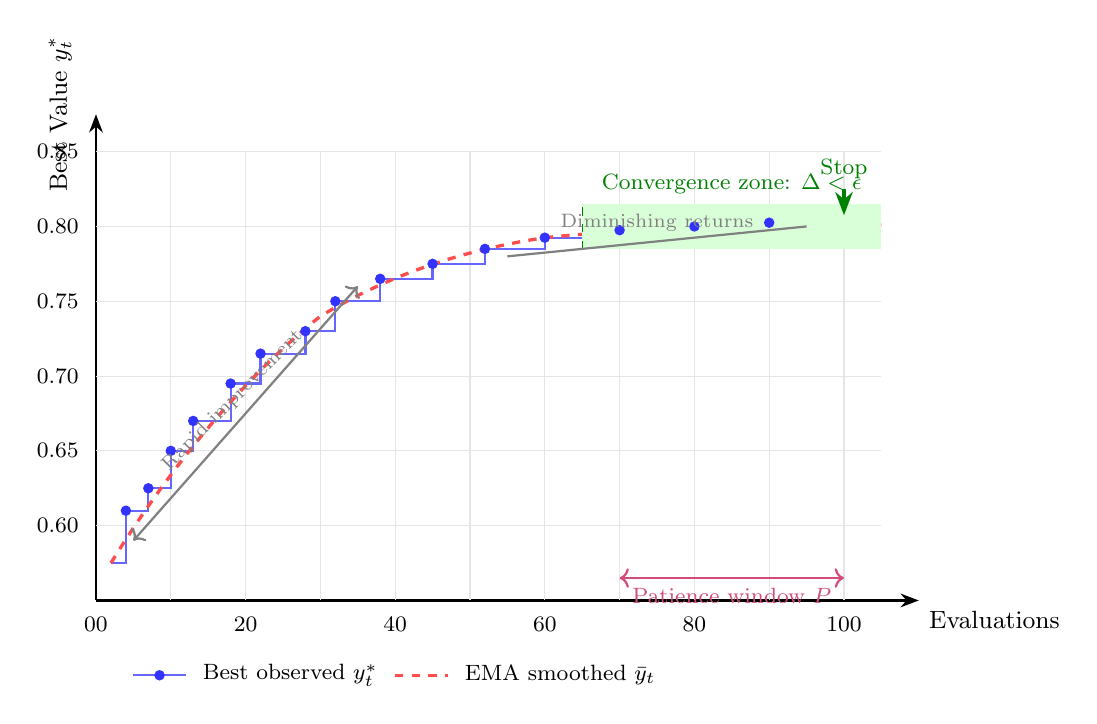
\begin{tikzpicture}[
    scale=0.95,
    every node/.style={font=\small}
]

% Axes
\draw[-{Stealth}, thick] (0,0) -- (11,0) node[anchor=north west] {Evaluations};
\draw[-{Stealth}, thick] (0,0) -- (0,6.5) node[anchor=south, rotate=90, yshift=5pt] {Best Value $y_t^*$};

% Grid
\foreach \x in {1,2,...,10} {
    \draw[gray!20] (\x, 0) -- (\x, 6);
}
\foreach \y in {1,2,...,6} {
    \draw[gray!20] (0, \y) -- (10.5, \y);
}

% X-axis labels
\foreach \x in {0,2,4,6,8,10} {
    \node[anchor=north, font=\footnotesize] at (\x, -0.1) {\x 0};
}

% Y-axis labels
\node[anchor=east, font=\footnotesize] at (-0.1, 1) {0.60};
\node[anchor=east, font=\footnotesize] at (-0.1, 2) {0.65};
\node[anchor=east, font=\footnotesize] at (-0.1, 3) {0.70};
\node[anchor=east, font=\footnotesize] at (-0.1, 4) {0.75};
\node[anchor=east, font=\footnotesize] at (-0.1, 5) {0.80};
\node[anchor=east, font=\footnotesize] at (-0.1, 6) {0.85};

% Raw best values (noisy, step function)
\draw[blue!60, thick]
    (0.2, 0.5) -- (0.4, 0.5) -- (0.4, 1.2) -- (0.7, 1.2) -- (0.7, 1.5)
    -- (1.0, 1.5) -- (1.0, 2.0) -- (1.3, 2.0) -- (1.3, 2.4)
    -- (1.8, 2.4) -- (1.8, 2.9) -- (2.2, 2.9) -- (2.2, 3.3)
    -- (2.8, 3.3) -- (2.8, 3.6) -- (3.2, 3.6) -- (3.2, 4.0)
    -- (3.8, 4.0) -- (3.8, 4.3) -- (4.5, 4.3) -- (4.5, 4.5)
    -- (5.2, 4.5) -- (5.2, 4.7) -- (6.0, 4.7) -- (6.0, 4.85)
    -- (7.0, 4.85) -- (7.0, 4.95) -- (8.0, 4.95) -- (8.0, 5.0)
    -- (9.0, 5.0) -- (9.0, 5.05) -- (10.5, 5.05);

% EMA smoothed curve
\draw[red!70, very thick, dashed]
    (0.2, 0.5) .. controls (1, 1.8) and (2, 3.0) .. (3, 3.8)
    .. controls (4, 4.4) and (5, 4.7) .. (6, 4.85)
    .. controls (7, 4.95) and (8, 5.0) .. (10.5, 5.02);

% Convergence threshold zone
\fill[green!15] (6.5, 4.7) rectangle (10.5, 5.3);
\draw[green!50!black, dashed] (6.5, 4.7) -- (6.5, 5.3);
\node[green!50!black, font=\footnotesize, anchor=south] at (8.5, 5.3) {Convergence zone: $\Delta < \epsilon$};

% Patience window
\draw[<->, purple!70, thick] (7, 0.3) -- (10, 0.3);
\node[purple!70, font=\footnotesize, anchor=north] at (8.5, 0.3) {Patience window $P$};

% Improvement markers
\foreach \x/\y in {0.4/1.2, 0.7/1.5, 1.0/2.0, 1.3/2.4, 1.8/2.9, 2.2/3.3, 2.8/3.6, 3.2/4.0, 3.8/4.3, 4.5/4.5, 5.2/4.7, 6.0/4.85, 7.0/4.95, 8.0/5.0, 9.0/5.05} {
    \fill[blue!80] (\x, \y) circle (2pt);
}

% Convergence detected marker
\draw[green!50!black, very thick, -{Stealth}] (10, 5.5) -- (10, 5.15);
\node[green!50!black, font=\footnotesize, anchor=south] at (10, 5.5) {Stop};

% Legend
\draw[blue!60, thick] (0.5, -1) -- (1.2, -1);
\fill[blue!80] (0.85, -1) circle (2pt);
\node[anchor=west, font=\footnotesize] at (1.3, -1) {Best observed $y_t^*$};

\draw[red!70, very thick, dashed] (4, -1) -- (4.7, -1);
\node[anchor=west, font=\footnotesize] at (4.8, -1) {EMA smoothed $\bar{y}_t$};

% Annotation for rapid improvement
\draw[<->, gray, thick] (0.5, 0.8) -- (3.5, 4.2);
\node[gray, font=\scriptsize, anchor=south, rotate=45] at (2, 2.5) {Rapid improvement};

% Annotation for diminishing returns
\draw[gray, thick] (5.5, 4.6) -- (9.5, 5);
\node[gray, font=\scriptsize, anchor=south] at (7.5, 4.8) {Diminishing returns};

\end{tikzpicture}
\end{document}
